\chapter{Sprint 1: Authentication and User Management}
\section{Introduction}
In the first sprint of our project we decided to start with the basics, setting up the authentication system and
handle features related to user management. Finishing this sprint will allow us to have a solid foundation for the
rest of the project since it will allow us to manage the users and their roles in the platform.

\section{Backlog Sprint}
Following the scrum framework, we have defined the sprint backlog for the first sprint.
The following table shows the user stories and their corresponding tasks that will be developed in this sprint.
Being a team, we distributed these task among us, so that each member of the team is responsible for a set of tasks.

\normalsize
\begin{longtable}{|p{1cm}|p{7cm}|p{1cm}|p{7cm}|}
    \hline
    \rowcolor{green!20} \textbf{ID} & \textbf{User Story}                                           & \textbf{ID} & \textbf{Tasks}                        \\ \hline
    1                               & As a platform user, I want to login to the platform           & 1.1         & Create user interface                 \\ \cline{3-4}
                                    &                                                               & 1.2         & Handle input validation and API calls \\ \cline{3-4}
                                    &                                                               & 1.3         & Implement needed APIs                 \\ \cline{3-4}
                                    &                                                               & 1.4         & Test the feature                      \\ \hline
    2                               & As a platform user, I want to update my profile               & 2.1         & Create user interface                 \\ \cline{3-4}
                                    &                                                               & 2.2         & Handle input validation and API calls \\ \cline{3-4}
                                    &                                                               & 2.3         & Implement needed APIs                 \\ \cline{3-4}
                                    &                                                               & 2.4         & Test the feature                      \\ \hline
    3                               & As a platform user, I want to logout of the platform          & 3.1         & Create user interface                 \\ \cline{3-4}
                                    &                                                               & 3.2         & Handle input validation and API calls \\ \cline{3-4}
                                    &                                                               & 3.3         & Implement needed APIs                 \\ \cline{3-4}
                                    &                                                               & 3.4         & Test the feature                      \\ \hline
    4                               & As a platform user, I want to change my password              & 4.1         & Create user interface                 \\ \cline{3-4}
                                    &                                                               & 4.2         & Handle input validation and API calls \\ \cline{3-4}
                                    &                                                               & 4.3         & Implement needed APIs                 \\ \cline{3-4}
                                    &                                                               & 4.4         & Test the feature                      \\ \hline
    5                               & As a platform user, I want to view my profile                 & 5.1         & Create user interface                 \\ \cline{3-4}
                                    &                                                               & 5.2         & Handle input validation and API calls \\ \cline{3-4}
                                    &                                                               & 5.3         & Implement needed APIs                 \\ \cline{3-4}
                                    &                                                               & 5.4         & Test the feature                      \\ \hline
    6                               & As a super admin, I want to add a new ODC Coordinator         & 6.1         & Create user interface                 \\ \cline{3-4}
                                    &                                                               & 6.2         & Handle input validation and API calls \\ \cline{3-4}
                                    &                                                               & 6.3         & Implement needed APIs                 \\ \cline{3-4}
                                    &                                                               & 6.4         & Test the feature                      \\ \hline
    7                               & As a super admin, I want to view ODC Coordinators list        & 7.1         & Create user interface                 \\ \cline{3-4}
                                    &                                                               & 7.2         & Handle input validation and API calls \\ \cline{3-4}
                                    &                                                               & 7.3         & Implement needed APIs                 \\ \cline{3-4}
                                    &                                                               & 7.4         & Test the feature                      \\ \hline
    8                               & As a super admin, I want to enable/disable an ODC Coordinator & 8.1         & Create user interface                 \\ \cline{3-4}
                                    &                                                               & 8.2         & Handle input validation and API calls \\ \cline{3-4}
                                    &                                                               & 8.3         & Implement needed APIs                 \\ \cline{3-4}
                                    &                                                               & 8.4         & Test the feature                      \\ \hline
    9                               & As an ODC Coordinator, I want to add a new ODC Expert         & 9.1         & Create user interface                 \\ \cline{3-4}
                                    &                                                               & 9.2         & Handle input validation and API calls \\ \cline{3-4}
                                    &                                                               & 9.3         & Implement needed APIs                 \\ \cline{3-4}
                                    &                                                               & 9.4         & Test the feature                      \\ \hline
    10                              & As an ODC Coordinator, I want to view ODC Experts list        & 10.1        & Create user interface                 \\ \cline{3-4}
                                    &                                                               & 10.2        & Handle input validation and API calls \\ \cline{3-4}
                                    &                                                               & 10.3        & Implement needed APIs                 \\ \cline{3-4}
                                    &                                                               & 10.4        & Test the feature                      \\ \hline
    11                              & As an ODC Coordinator, I want to enable/disable an ODC Expert & 11.1        & Create user interface                 \\ \cline{3-4}
                                    &                                                               & 11.2        & Handle input validation and API calls \\ \cline{3-4}
                                    &                                                               & 11.3        & Implement needed APIs                 \\ \cline{3-4}
                                    &                                                               & 11.4        & Test the feature                      \\ \hline
    \caption{Sprint Backlog for Authentication and User Management}
    \label{tab:sprint_backlog_auth_user_mgmt}
\end{longtable}


\section{Functional Requirements}
\subsection{Use Case Diagram}
The use case diagram in Figure \ref{fig:Use Case Diagram for Sprint 1} shows the use cases that we defined for the first sprint.
The main use cases are related to the authentication and user management features. The actors are the users of the platform,
which can be either a collaborator or an administrator.

\begin{figure}[h!]
    \centering
    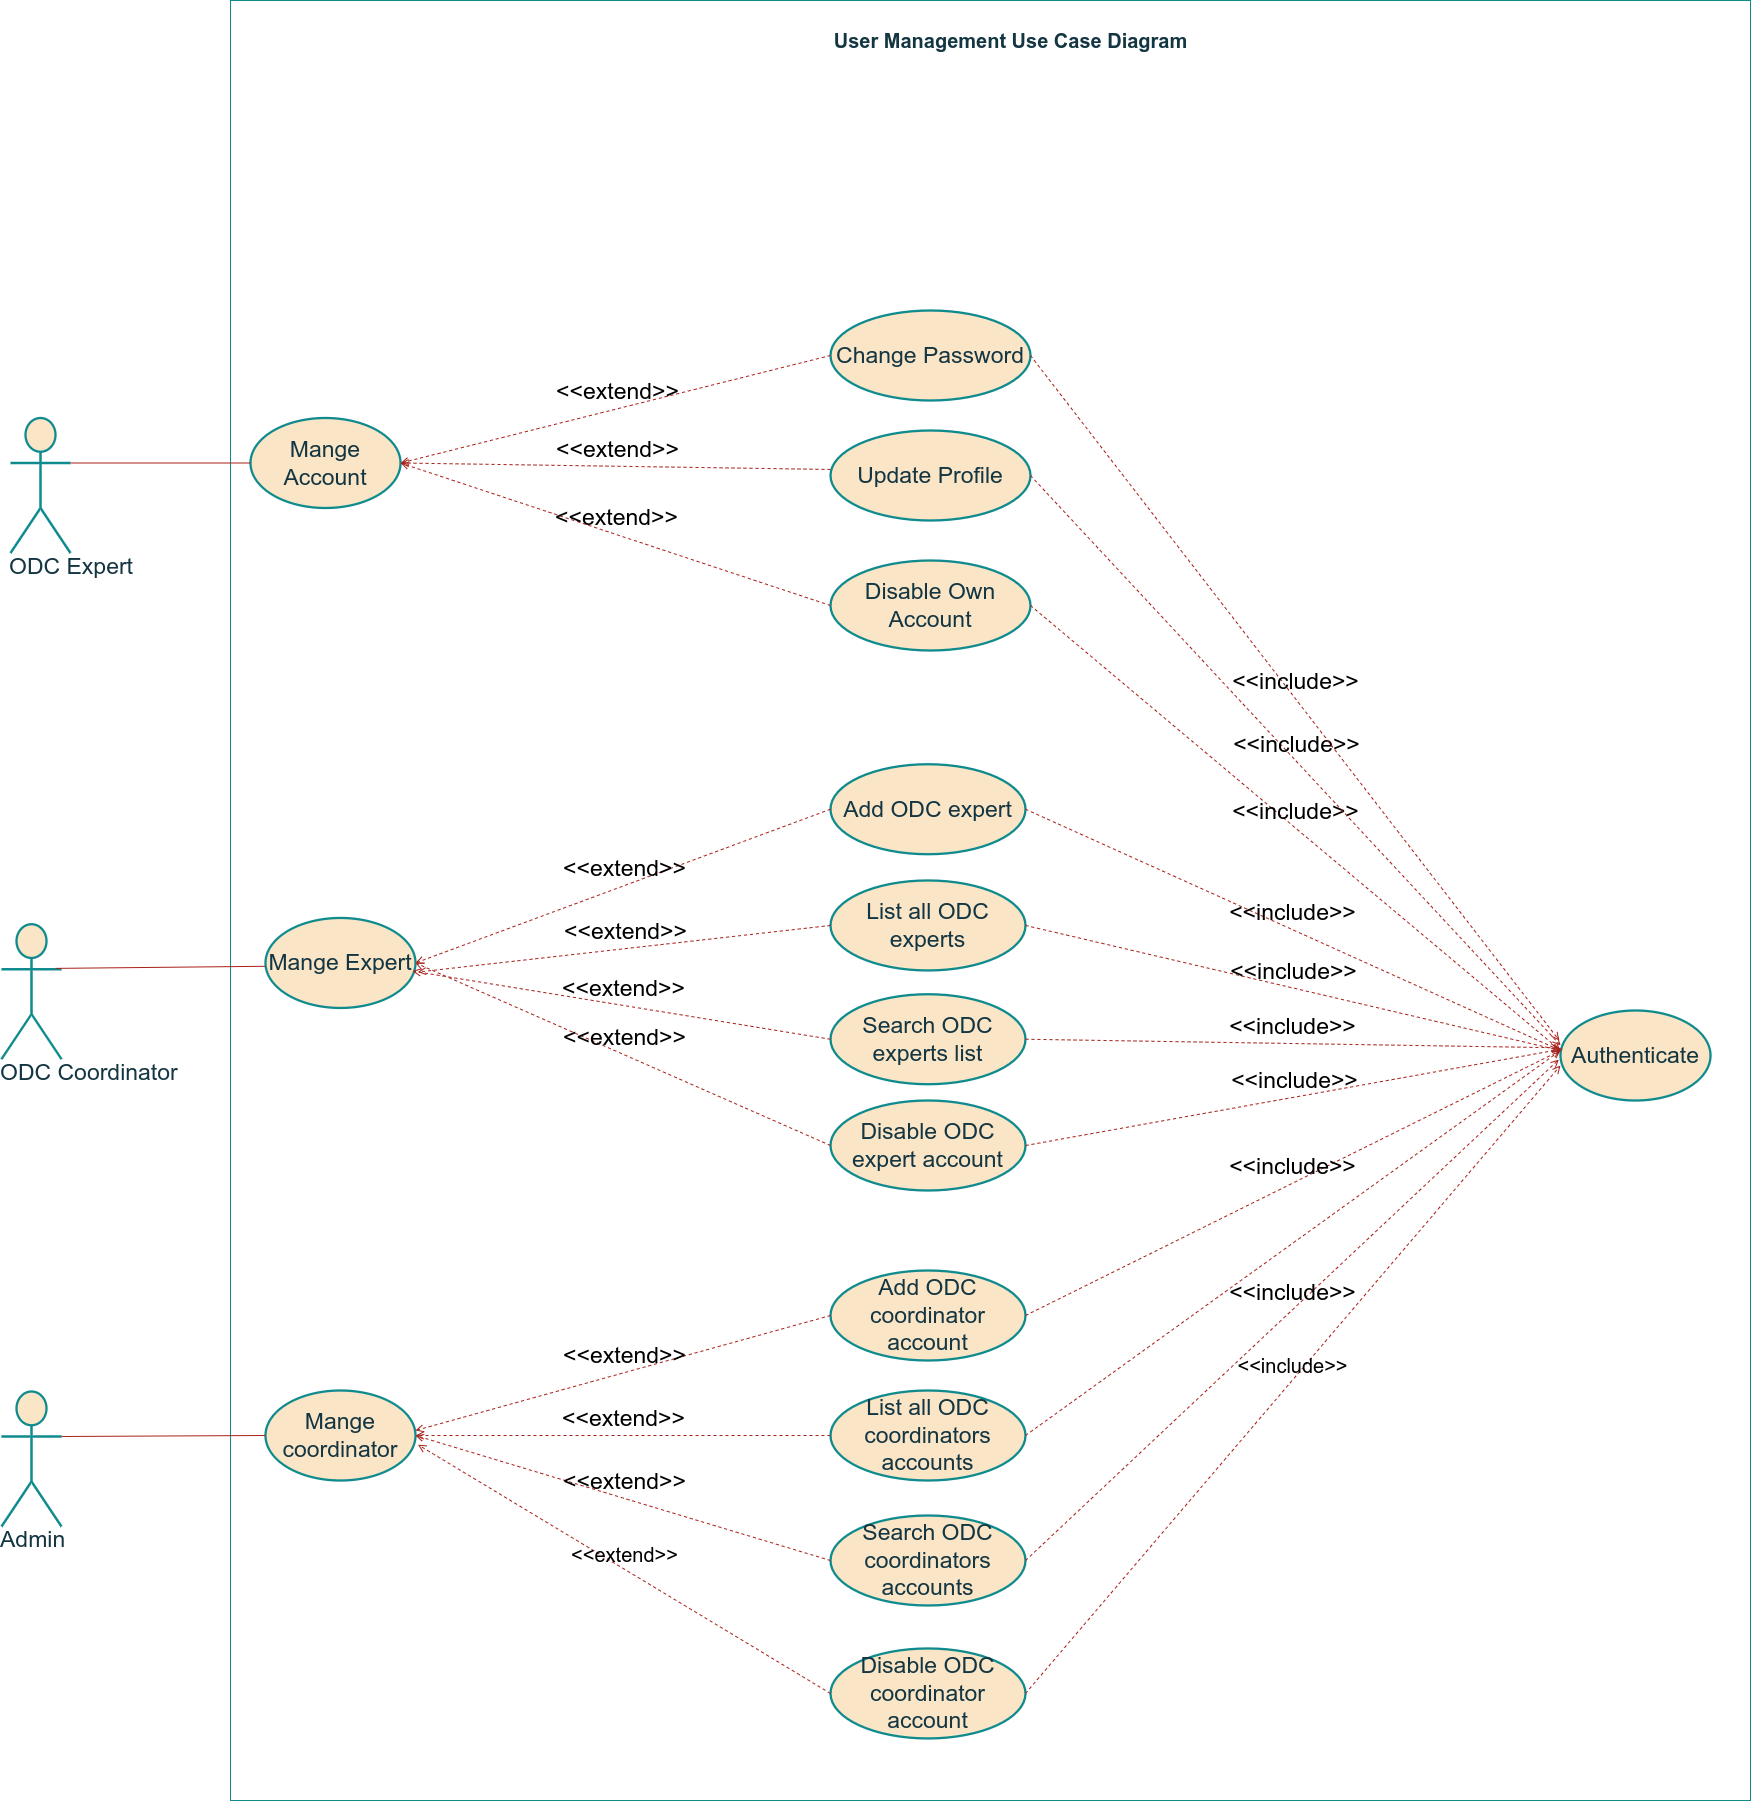
\includegraphics[height=1\textwidth]{images/userManagementUseCase.png}
    \caption{Use Case Diagram For The Authentication and User Management Sprint}
    \label{fig:Use Case Diagram for Sprint 1}
\end{figure}

\subsection{Textual Description Of The Login Use Case}
The login use case is the most important use case in this sprint. It allows the user to authenticate in the platform.
The following table shows the textual description of the login use case.

\begin{table}[h]
    \centering
    \renewcommand{\arraystretch}{2} % Adjust the line height here
    \begin{tabular}{|p{3cm}|p{12cm}|}
        \hline
        \rowcolor{green!20} \textbf{Use Case} & Login                                                                                                              \\
        \hline
        \textbf{Actor}                        & User: Collaborator/Administrator                                                                                   \\
        \hline
        \textbf{Brief Description}            & The user must be registered in the database and must know their credentials                                        \\
        \hline
        \textbf{Pre-condition}                & The user must have their access parameters                                                                         \\
        \hline
        \textbf{Post-condition}               & The user is successfully authenticated                                                                             \\
        \hline
        \textbf{Main Scenario}                & 1. The user enters their credentials (email and password) in the appropriate fields and submits the form. \newline
        2. The system verifies the information entered by the user. \newline
        3. The system displays the appropriate interface according to the role of the user.                                                                        \\
        \hline
        \textbf{Exception Scenario}           & 1.1 The entered data is incorrect or missing: \newline
        1.1.1 The system displays an error message and the use case returns to step 1 of the main scenario. \newline
        2.1 The entered credentials do not exist in the database: \newline
        2.1.1 The system displays an error message and the use case returns to step 2 of the main scenario.                                                        \\
        \hline
        \textbf{Extension}                    & In case of forgotten password, the user can redefine a new password                                                \\
        \hline
    \end{tabular}
    \caption{Textual Description of the Use Case `Login`}
    \label{tab:Textual_Description_of_the_Use_Case_Authenticate}
\end{table}

\subsection{Textual Description Of The Use Case `Add Coordinator`}
Adding a new coordinator is a use case that is only available to the super admin. The following table shows the textual description
of the steps that the super admin must follow to add a new coordinator to the platorm.

\begin{table}[h]
    \centering
    \renewcommand{\arraystretch}{1.5} % Adjust the line height here
    \begin{tabular}{|p{3cm}|p{12cm}|}
        \hline
        \rowcolor{green!20} \textbf{Use Case} & Add Coordinator                                                                                                                        \\
        \hline
        \textbf{Actor}                        & \begin{tabular}[t]{@{}l@{}}
                                                    Super Admin \\
                                                    Coordinator
                                                \end{tabular}                                                                                                             \\
        \hline
        \textbf{Brief Description}            & The Super Admin adds a new coordinator by providing the necessary details. The coordinator receives an email to set up their password. \\
        \hline
        \textbf{Pre-condition}                & The Super Admin must be authenticated and have the necessary permissions.                                                              \\
        \hline
        \textbf{Post-condition}               & The coordinator is successfully added and can log in after setting up their password.                                                  \\
        \hline
        \textbf{Main Scenario}                & \begin{tabular}[t]{@{}l@{}}
                                                    1. The Super Admin accesses the "Add New Coordinator" page.  \\
                                                    2. The Super Admin fills in the fields: name,                \\ last name, country, email. \\
                                                    3. The Super Admin presses the "Add" button.                 \\
                                                    4. The system validates the entered information.             \\
                                                    5. The system sends an email to the new coordinator.         \\
                                                    6. The coordinator receives the email and clicks the link.   \\
                                                    7. The coordinator is redirected to the password setup page. \\
                                                    8. The coordinator sets up the password.                     \\
                                                    9. The coordinator is redirected to the login page.
                                                \end{tabular}                                             \\
        \hline
        \textbf{Exception Scenario}           & \begin{tabular}[t]{@{}l@{}}
                                                    2.1 The entered data is incorrect or missing:               \\
                                                    2.1.1 The system displays an error message and the use case \\ returns to step 2. \\
                                                    4.1 The entered email is already in use or invalid:         \\
                                                    4.1.1 The system displays an error message and the use case \\ returns to step 2.
                                                \end{tabular}                                                      \\
        \hline
        \textbf{Extension}                    & In case of forgotten password, the coordinator can redefine a new password.                                                            \\
        \hline
    \end{tabular}
    \caption{Textual Description of the Use Case "Add Coordinator"}
    \label{tab:Textual_Description_of_the_Use_Case_Add_Coordinator}
\end{table}

\subsection{Textual Description of the Use Case `Enable/Disable ODC Expert`}
\begin{table}[h]
    \centering
    \renewcommand{\arraystretch}{1.5}
    \begin{tabular}{|p{3cm}|p{12cm}|}
        \hline
        \rowcolor{green!20} \textbf{Use Case} & Enable/Disable ODC Expert                                                                                                                                                                                                                                                \\
        \hline
        \textbf{Actor}                        & ODC Coordinator                                                                                                                                                                                                                                                          \\
        \hline
        \textbf{Brief Description}            & The ODC Coordinator wants to enable or disable an ODC Expert in the system. The Coordinator searches for the expert in the experts list and presses the button to enable or disable the expert. The system updates the `isEnabled` variable in the database accordingly. \\
        \hline
        \textbf{Pre-condition}                & The ODC Coordinator must have access to the system and there must be a list of experts in the system.                                                                                                                                                                    \\
        \hline
        \textbf{Post-condition}               & The `isEnabled` status of the expert is updated in the database.                                                                                                                                                                                                         \\
        \hline
        \textbf{Main Scenario}                & \begin{tabular}[l]{@{}l@{}}
                                                    1. The ODC Coordinator accesses the system and                \\searches for the expert in the experts list. \\
                                                    2. The ODC Coordinator presses the enable/disable button      \\ corresponding to the expert. \\
                                                    3. The system sends a request to the database to update the   \\ `isEnabled` variable for the expert. \\
                                                    4. The database updates the `isEnabled` variable to `true` if \\ enabling or `false` if disabling. \\
                                                    5. The database confirms the update to the system.            \\
                                                    6. The system displays the updated status (enabled/disabled)  \\ to the ODC Coordinator.
                                                \end{tabular}                                                                                                                                                             \\
        \hline
        \textbf{Exception Scenario}           & \begin{tabular}[l]{@{}l@{}}
                                                    1. The entered expert is not found:                           \\
                                                    - The system displays a message indicating that no expert was \\found in the list. \\
                                                    2. Database update failure:                                   \\
                                                    - The system displays an error message indicating the failure.
                                                \end{tabular}                                                                                                                                                                                       \\
        \hline
        \textbf{Extension}                    & If the search query is invalid or empty, the system prompts the ODC Coordinator to enter a valid query. If the system is unable to connect to the database, an error message is displayed and the operation is aborted.                                                  \\
        \hline
    \end{tabular}
    \caption{Textual Description of the Use Case "Enable/Disable ODC Expert"}
    \label{tab:Textual_Description_of_the_Use_Case_Enable_Disable_ODC_Expert}
\end{table}


\section{Analysis And Design}
In this section, we will present the decisions that we made regarding the implementation
of the features related to authentication and user management.

\subsection{Database Design}
When Building an application, it is important to have a good authentication system in place.
We decided to implement our own system that it will be based on the following schema \ref{fig:Database Schema}.

\begin{figure}[h!]
    \centering
    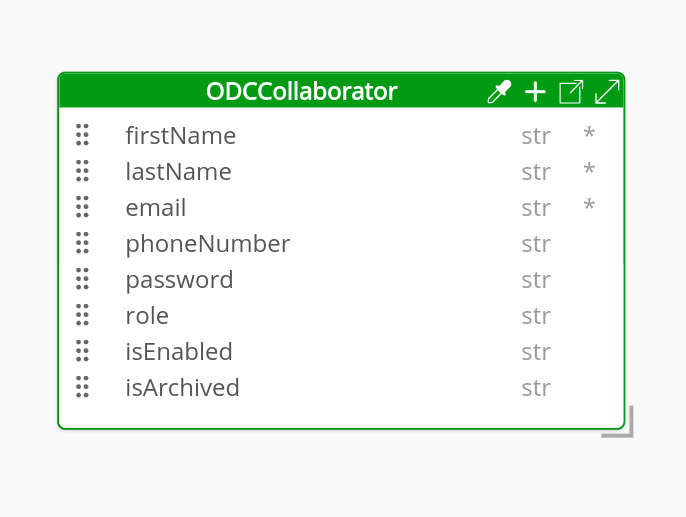
\includegraphics[width=1\textwidth]{images/diagram-ODCCollaborator.png}
    \caption{ODC Collaborator Database Schema}
    \label{fig:Database Schema}
\end{figure}

As an authentication mechanism, we implemented a stateless JWT (JSON Web Token) authentication system.
where the user well be authenticated by providing their email and password, and if the credentials are correct,
the server will return a token that the user can use to authenticate in the platform.

For password management, we decided to use the bcrypt hashing algorithm to hash the password before storing it in the database.
This will ensure that the password is secure and cannot be decrypted.

To authorization and access control, we assigned a role to each user. the roles are defined as follows:
\begin{itemize}
    \item Super Admin
    \item Coordinator
    \item Expert
\end{itemize}

Any request to the server will be validated by checking the role of the user and the permissions that the user has.
For example, only the super admin can add a new coordinator, and only the coordinator can add a new expert.
If the user tries to access a resource that they are not allowed to, the server will return a 403 Forbidden error.

The sequence diagram in Figure \ref{fig:Login Sequence Diagram for ODC Collaborator} shows the steps that the user must follow to authenticate in the platform.
It is valid for all the users of the platform.

\begin{figure}
    \centering
    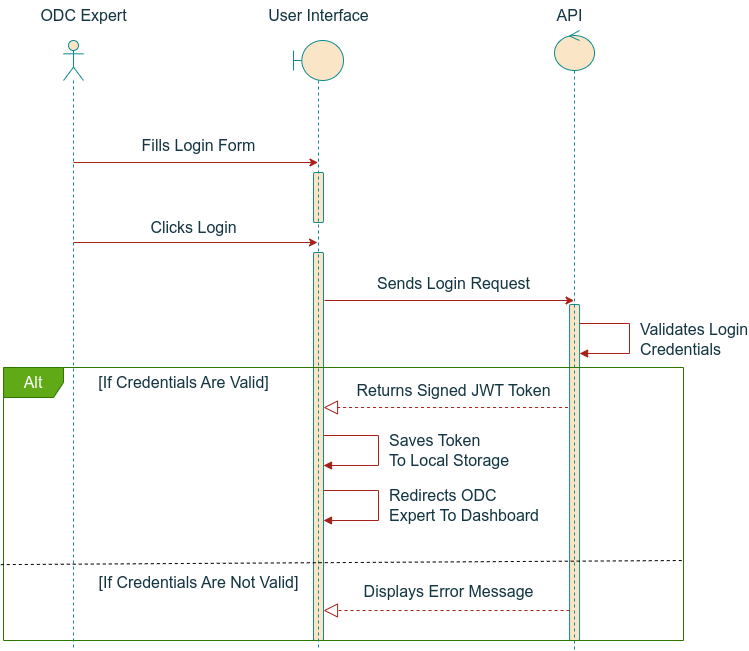
\includegraphics[width=1\textwidth]{images/sequenceODCExpertLogin.png}
    \caption{Login Sequence Diagram for ODC Expert}
    \label{fig:Login Sequence Diagram for ODC Expert}
\end{figure}

When Adding a new ODC Coordinator or Expert, the super admin or the coordinator must provide the necessary information.
The system will validate the information and send an email to the new user to set up their password.

The sequence diagram in Figure \ref{fig:Add ODC Expert Sequence Diagram} shows
the steps that the ODC Coordinator must follow to add a new coordinator to the
platform.

\begin{figure}[h!]
    \centering
    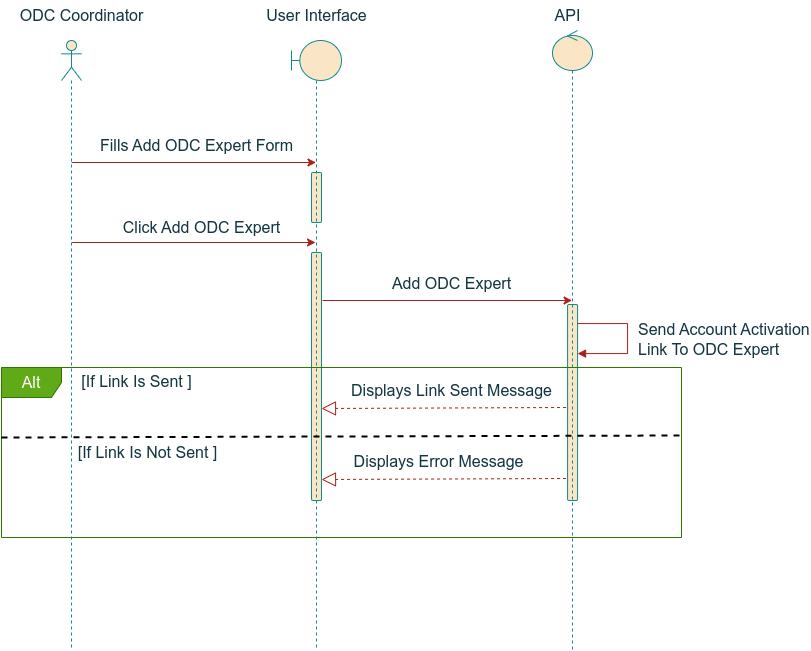
\includegraphics[width=1\textwidth]{images/sequenceAddODCExpert.png}
    \caption{Add ODC Expert Sequence Diagram}
    \label{fig:Add ODC Expert Sequence Diagram}
\end{figure}

\newpage
After Adding a new coordinator, the system will send an email to the new coordinator with a link to set up their password.
The sequence diagram in Figure \ref{fig:Activate Account Sequence Diagram} shows the steps that the ODC Expert must follow
to activate their account.

\begin{figure}[h!]
    \centering
    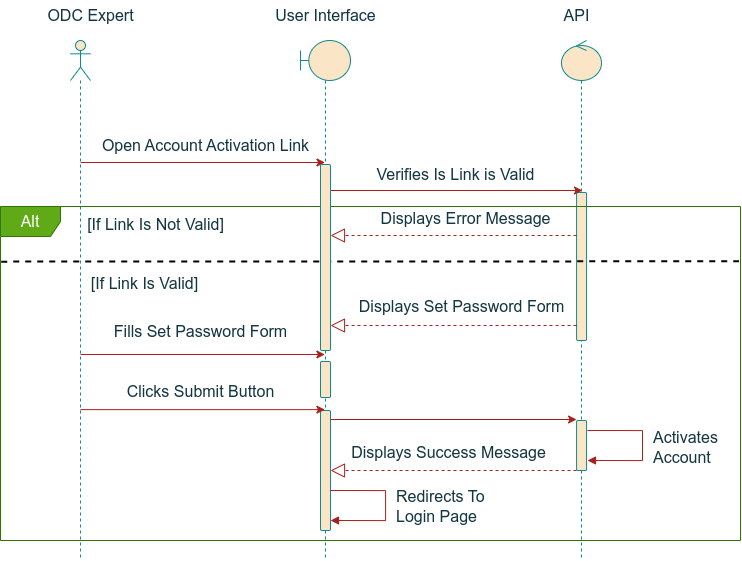
\includegraphics[width=1\textwidth]{images/sequenceActivateAccount.png}
    \caption{Activate Account Sequence Diagram}
    \label{fig:Active Account Sequence Diagram}
\end{figure}

\section{Implementation}
